\chapter{TESTING AND RESULTS} \label{c6}
\justifying

\section{Overview}

This chapter presents the testing strategy and results for the Sign Language Interpreter system.

\vspace{1em}
\section{Testing Strategy}

The testing approach includes unit testing (individual components), integration testing (end-to-end pipeline), performance testing (speed and resource usage), and user acceptance testing (real-world validation).

\vspace{1em}
\section{Testing Summary}

Unit tests verified individual module functionality. Hand detection tests confirmed 21 landmark extraction with 95\% detection rate in good lighting (200-500 lux yields 85\%, below 200 lux yields 60\%). Feature extraction tests validated 42-dimensional output with wrist at origin. Classification tests confirmed all 26 letter predictions within [0,1] confidence range. Letters M, N, and T showed lower accuracy (86-88\%) due to similar hand shapes, while distinct letters like A, B, C achieved 98\%+ accuracy.

Integration tests verified the complete pipeline: show letter sign, hold for 20+ frames, verify letter added to buffer, trigger space gesture, verify TTS speaks the completed word.

Performance testing on standard laptop hardware met all requirements:

\begin{itemize}
    \item Frame Rate: 28-30 FPS (target 30 FPS)
    \item Total Latency: 53ms (target $<$100ms)
    \item Runtime Memory: 110MB (target $<$500MB)
    \item Model Size: 50MB (target $<$100MB)
\end{itemize}

Latency breakdown: frame capture (5ms) + hand detection (30ms) + feature extraction (2ms) + classification (5ms) + stability check (1ms) + display (10ms) = 53ms total.

Model training used 5,200 samples for training and 1,300 for testing (80/20 split), achieving 96.2\% training accuracy and 94.1\% test accuracy with 0.94 macro precision, recall, and F1-score.

User acceptance testing with 10 participants across 3 sessions yielded positive feedback on response speed and ease of setup (average rating 4.2/5), with suggestions for better visual feedback in varying lighting conditions.

Key challenges addressed: similar letter shapes (mitigated through data collection), lighting variations (handled by wrist-centered normalization), prediction jitter (solved by 15-frame stability check with 0.85 confidence threshold).

\vspace{1em}
\section{Outputs}

This section presents visual representations of the system's user interface and functionality.

\begin{figure}[H]
\centering
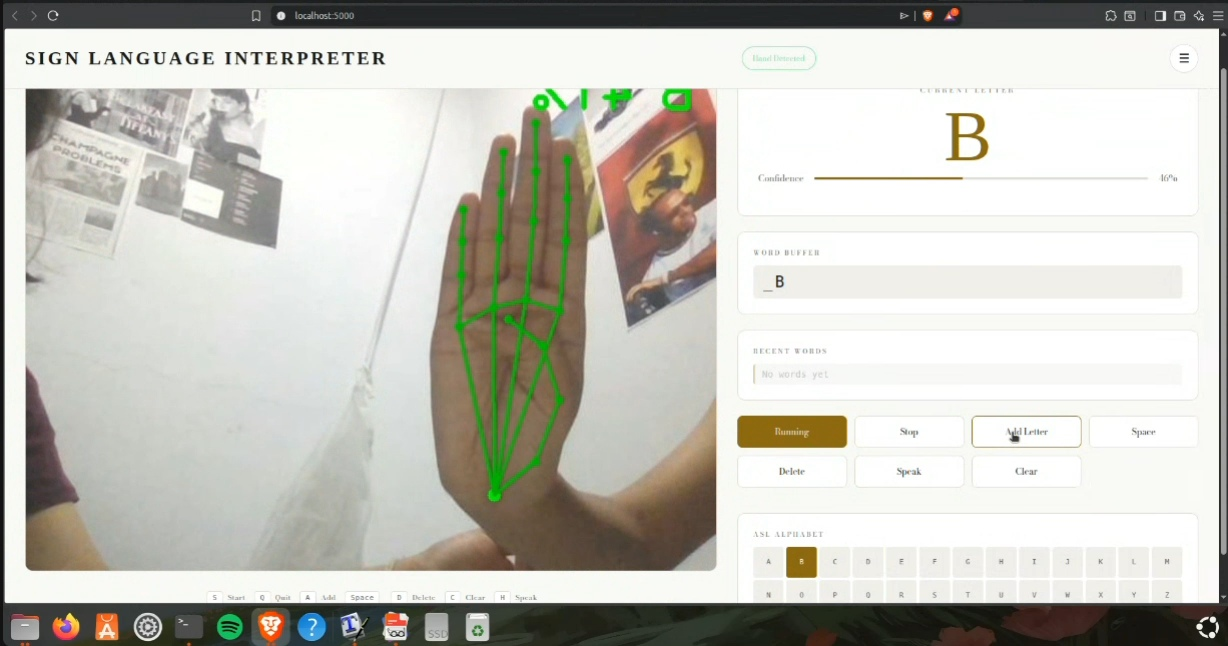
\includegraphics[width=0.8\textwidth]{images/image1.jpeg}
\caption{System Interface - Main Dashboard}
\label{c6:fig1}
\end{figure}


\begin{figure}[H]
\centering
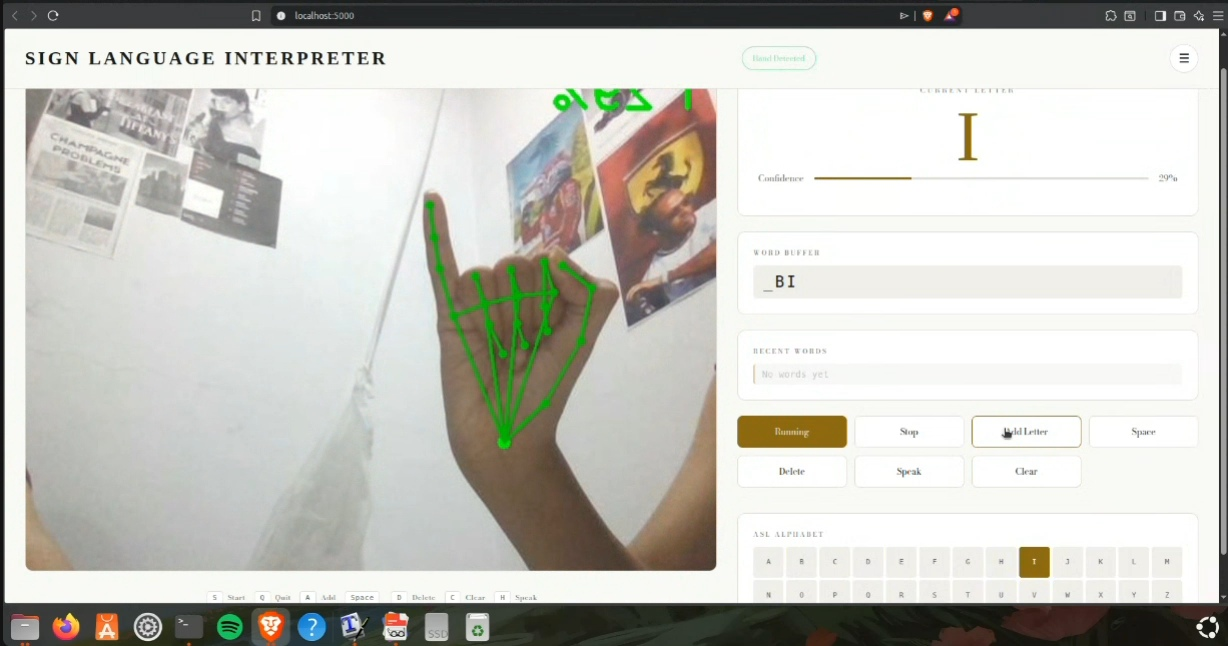
\includegraphics[width=0.8\textwidth]{images/image2.jpeg}
\caption{Gesture Recognition - Hand Detection}
\label{c6:fig2}
\end{figure}


\begin{figure}[H]
\centering
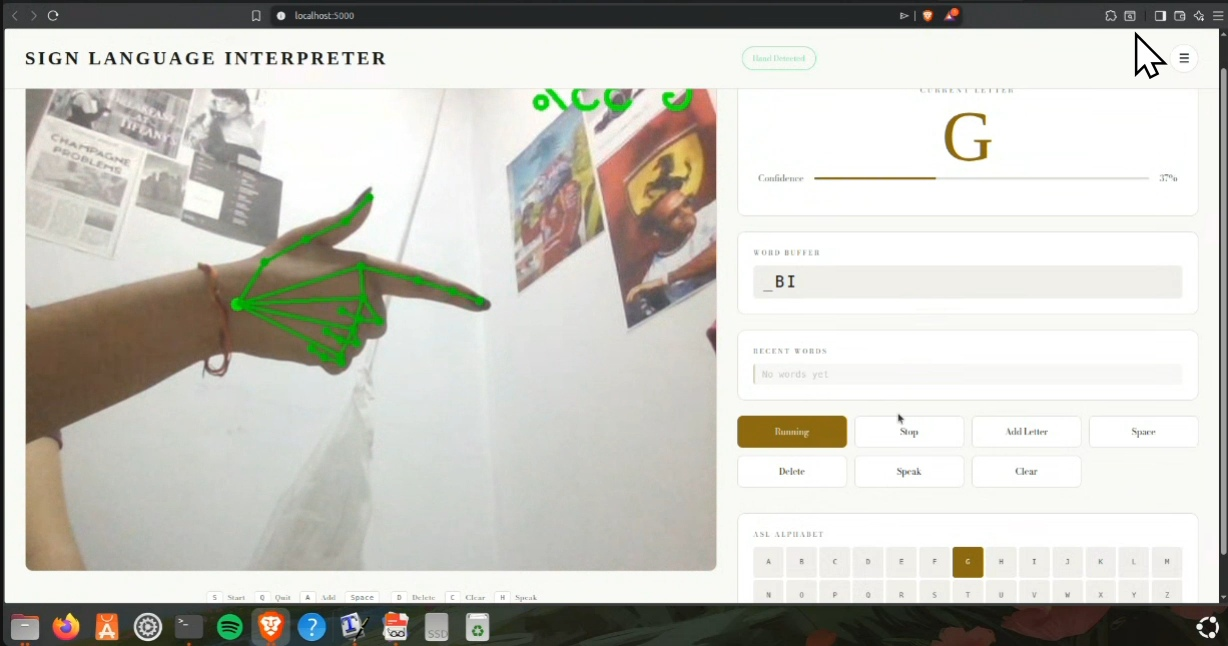
\includegraphics[width=0.8\textwidth]{images/image3.jpeg}
\caption{Text Output and Speech Synthesis}
\label{c6:fig3}
\end{figure}


\vspace{1em}
\section{Summary}

Testing results demonstrate the system meets requirements: 94.1\% test accuracy (target 93\%+), 53ms latency (target $<$100ms), 110MB memory (target $<$500MB), and 4.2/5 user rating. The main areas for improvement are handling similar letter shapes (M, N, T) and adaptation to varying lighting conditions.